\documentclass[aps,prl,twocolumn,amsmath,amssymb,nofootinbib,superscriptaddress]{revtex4}

\newcommand{\bra}[1]{\langle#1|}
\newcommand{\ket}[1]{|#1\rangle}
\newcommand{\ip}[2]{\langle{#1}|{#2}\rangle}
\newcommand{\op}[2]{\hat{\textbf{#1}}_{#2}}
\newcommand{\dagop}[2]{\hat{\textbf{#1}}_{#2}^\dag}
\newcommand{\keith}[1]{{\color{cyan}{#1}}}
\newcommand{\peter}[1]{{\color{blue}{#1}}}
\newcommand{\daniel}[1]{{\color{magenta}{#1}}}
\newcommand{\remove}[1]{{\color{red}{#1}}}
\usepackage[pdftex]{graphicx}
\usepackage{mathrsfs}
\usepackage[usenames,dvipsnames]{color}
\usepackage[colorlinks]{hyperref}
\usepackage{comment}

\begin{document}

\bibliographystyle{apsrev}

\title{Cats doing algebra}

\author{Keith R. Motes}
\affiliation{Centre for Engineered Quantum Systems, Department of Physics \& Astronomy, Macquarie University, Sydney NSW 2113, Australia}

\author{Paul Knott}
\affiliation{NTT Basic Research Laboratories, NTT Corporation, Atsugi, Kanagawa 243-0198, Japan}

\author{William J. Munro}
\affiliation{NTT Basic Research Laboratories, NTT Corporation, Atsugi, Kanagawa 243-0198, Japan}

\author{Peter P. Rohde}
\affiliation{Centre for Engineered Quantum Systems, Department of Physics \& Astronomy, Macquarie University, Sydney NSW 2113, Australia}
\email[]{dr.rohde@gmail.com}
\homepage{http://www.peterrohde.org}

\date{\today}

\frenchspacing

\begin{abstract}
\end{abstract}

\maketitle

\section{To do}

Figure out general breeding cats

Once we've finalised out formalism, let's explore what the Wigner functions look like for higher order cat states.

Dfine wigner functions: F[num]:= amp of n photon term in psi= delta(n-m) = exp[...]. Then write W[x,p,F].

plot these several higher order wigner functions

Sensitivity of different order cat states against decoherence, specifically loss. Let's plot purity vs loss for different cases.

\section{Defintion}

Let $D(\alpha)$ be the displacement operator of amplitude $\alpha$.
\begin{eqnarray}
D(\alpha) = \exp(\alpha a^\dag - \alpha^* a)
\end{eqnarray}

Let us define two classes of cat operator: even (+) and odd (-),
\begin{equation}
A^\dag_\pm(\alpha) = D(\alpha) \pm D(-\alpha)
\end{equation}

To get the $A$ operators we use the property that $D^{\dag}(\alpha)=D(-\alpha)$,
\begin{eqnarray}
A_{\pm}(\alpha)=A_{\pm}^{\dag\dag}(\alpha)&=&D^{\dag}(\alpha)\pm D^{\dag}(-\alpha) \nonumber \\
&=&D(-\alpha)\pm D(\alpha).
\end{eqnarray}
We see that $A_+(\alpha)=A^{\dag}_+(\alpha)$ and $A_-(\alpha)=-A^{\dag}_-(\alpha)$.

Then we have
\begin{eqnarray}
A^\dag_\pm(\alpha) \ket{0} &=& \ket{\alpha} \pm \ket{-\alpha} \\
\bra{0}A_\pm(\alpha) &=& \pm \left(\bra{\alpha} \pm \bra{-\alpha}\right)
\end{eqnarray}

\section{Normalizations}
We will need the normalisation factors and calculate the four possibilities in this section. The normalised vector $\ket{\psi'}= \ket{\psi}/ \ip{\psi}{\psi}$. We must find each possible value of $\ip{\psi}{\psi}$. The four general possible combinations are $\bra{0}A_\pm(\alpha)A^\dag_\pm(\beta)\ket{0}$, which are calculated here,
\begin{eqnarray}
\bra{0}A_+(\alpha)A^\dag_+(\beta)\ket{0}&=& (\bra{\alpha}+\bra{-\alpha})(\ket{\beta}+\ket{-\beta}) \nonumber \\
&=& \ip{\alpha}{\beta}+\ip{\alpha}{-\beta}+\ip{-\alpha}{\beta}+\ip{-\alpha}{-\beta} \nonumber \\
&=& 2\left(\mathrm{Re}\left[\ip{\alpha}{\beta}\right]+\mathrm{Re}\left[\ip{\alpha}{-\beta}\right]\right) \nonumber \\
&=& 2 e^{-\frac{1}{2}(|\alpha|^2+|\beta|^2)}\mathrm{Re}\left[e^{\alpha^*\beta}+e^{-\alpha^*\beta} \right] \nonumber \\
&=& 2 e^{-\frac{1}{2}(|\alpha|^2+|\beta|^2)} 2\mathrm{Re}\left[e^{\alpha^*\beta}\right] \nonumber \\
&=& 4 e^{-\frac{1}{2}(|\alpha|^2+|\beta|^2)} \mathrm{Re}\left[e^{\alpha^*\beta}\right] \\
\bra{0}A_-(\alpha)A^\dag_-(\beta)\ket{0}&=& -\left(\bra{\alpha}-\bra{-\alpha})(\ket{\beta}-\ket{-\beta}\right) \nonumber \\
&=& -\left(\ip{\alpha}{\beta}-\ip{\alpha}{-\beta}-\ip{-\alpha}{\beta}+\ip{-\alpha}{-\beta}\right) \nonumber \\
&=& -2\left(\mathrm{Re}\left[\ip{\alpha}{\beta}\right]-\mathrm{Re}\left[\ip{\alpha}{-\beta}\right]\right) \nonumber \\
&=& -2 e^{-\frac{1}{2}(|\alpha|^2+|\beta|^2)}\mathrm{Re}\left[e^{\alpha^*\beta}-e^{-\alpha^*\beta} \right] \nonumber \\
&=& 2 e^{-\frac{1}{2}(|\alpha|^2+|\beta|^2)} 2\mathrm{Im}\left[e^{\alpha^*\beta}\right] \nonumber \\
&=& 4 e^{-\frac{1}{2}(|\alpha|^2+|\beta|^2)} \mathrm{Im}\left[e^{\alpha^*\beta}\right] \\
\bra{0}A_+(\alpha)A^\dag_-(\beta)\ket{0}&=& \bra{\alpha}+\bra{-\alpha})(\ket{\beta}-\ket{-\beta} \nonumber \\
&=& \ip{\alpha}{\beta}-\ip{\alpha}{-\beta}+\ip{-\alpha}{\beta}-\ip{-\alpha}{-\beta} \nonumber \\
&=& 0 \\
\bra{0}A_-(\alpha)A^\dag_+(\beta)\ket{0}&=& -\left(\bra{\alpha}-\bra{-\alpha})(\ket{\beta}+\ket{-\beta}\right) \nonumber \\
&=& -\left(\ip{\alpha}{\beta}+\ip{\alpha}{-\beta}-\ip{-\alpha}{\beta}-\ip{-\alpha}{-\beta}\right) \nonumber \\
&=& 0,
\end{eqnarray}
where the coherent state overlap $\ip{\alpha}{\beta}\equiv\mathrm{exp}\left[-1/2(|\alpha|^2+|\beta|^2 - 2\alpha^*\beta) \right] $ was used.



\section{Small $\alpha$ limit for the $A^\dag$ operator}

In the small $\alpha$ limit we have
\begin{eqnarray}
A^\dag_\pm(\alpha)  &=& (1+(\alpha a^\dag - \alpha^* a)) \pm (1+(-\alpha a^\dag + \alpha^* a)),\nonumber \\
\end{eqnarray}
because $e^{x}\approx 1+x$ for $x\ll1$.

For the even (+) case this reduces to,
\begin{eqnarray}
A^\dag_+(\alpha\to 0) = 2,
\end{eqnarray}
and for the odd (-) case this reduces to
\begin{eqnarray}
A^\dag_-(\alpha\to 0) = 2\alpha a^\dag - 2\alpha^* a.
\end{eqnarray}
Thus in the small $\alpha$ limit our $A^\dag_\pm$ does not reduce to the photonic creation operator.

\section{Commutation relations}

Since the cat operators may be expressed in terms of displacement operators, and displacement operators commute, 
\begin{eqnarray}
[D(\alpha),D(\beta)] &=& D(\alpha)D(\beta)-D(\beta)D(\alpha) \nonumber \\
&=& e^{i \mathrm{Im}[\alpha \beta^*]}D(\alpha+\beta)-e^{i \mathrm{Im}[\beta \alpha^*]}D(\alpha+\beta) \nonumber \\
&=& D(\alpha+\beta)\left(e^{i \mathrm{Im}[\alpha \beta^*]}- e^{i \mathrm{Im}[\beta \alpha^*]}\right).
\end{eqnarray}
This is zero if $\alpha$ and $\beta$ are real which is the case for the rest of this work. It follows that cat operators commute,
\begin{eqnarray}
[A_\pm^\dag(\alpha), A_\pm^\dag(\beta)] &=& 0 \\ \nonumber
[A_\pm^\dag(\alpha), A_\mp^\dag(\beta)] &=& 0 
\end{eqnarray}

\section{A cat basis}

Since,
\begin{equation}
A^\dag_+(\alpha) + A^\dag_-(\alpha) = 2D(\alpha)
\end{equation}
it follows that first order cat states can generate arbitrary coherent states, and thus, since coherent states form an overcomplete basis in the photon-number degree of freedom, it follows that cat states also form an overcomplete basis.

\section{Higher order cats}

%**********Figure*****************
\begin{figure}[!htb]
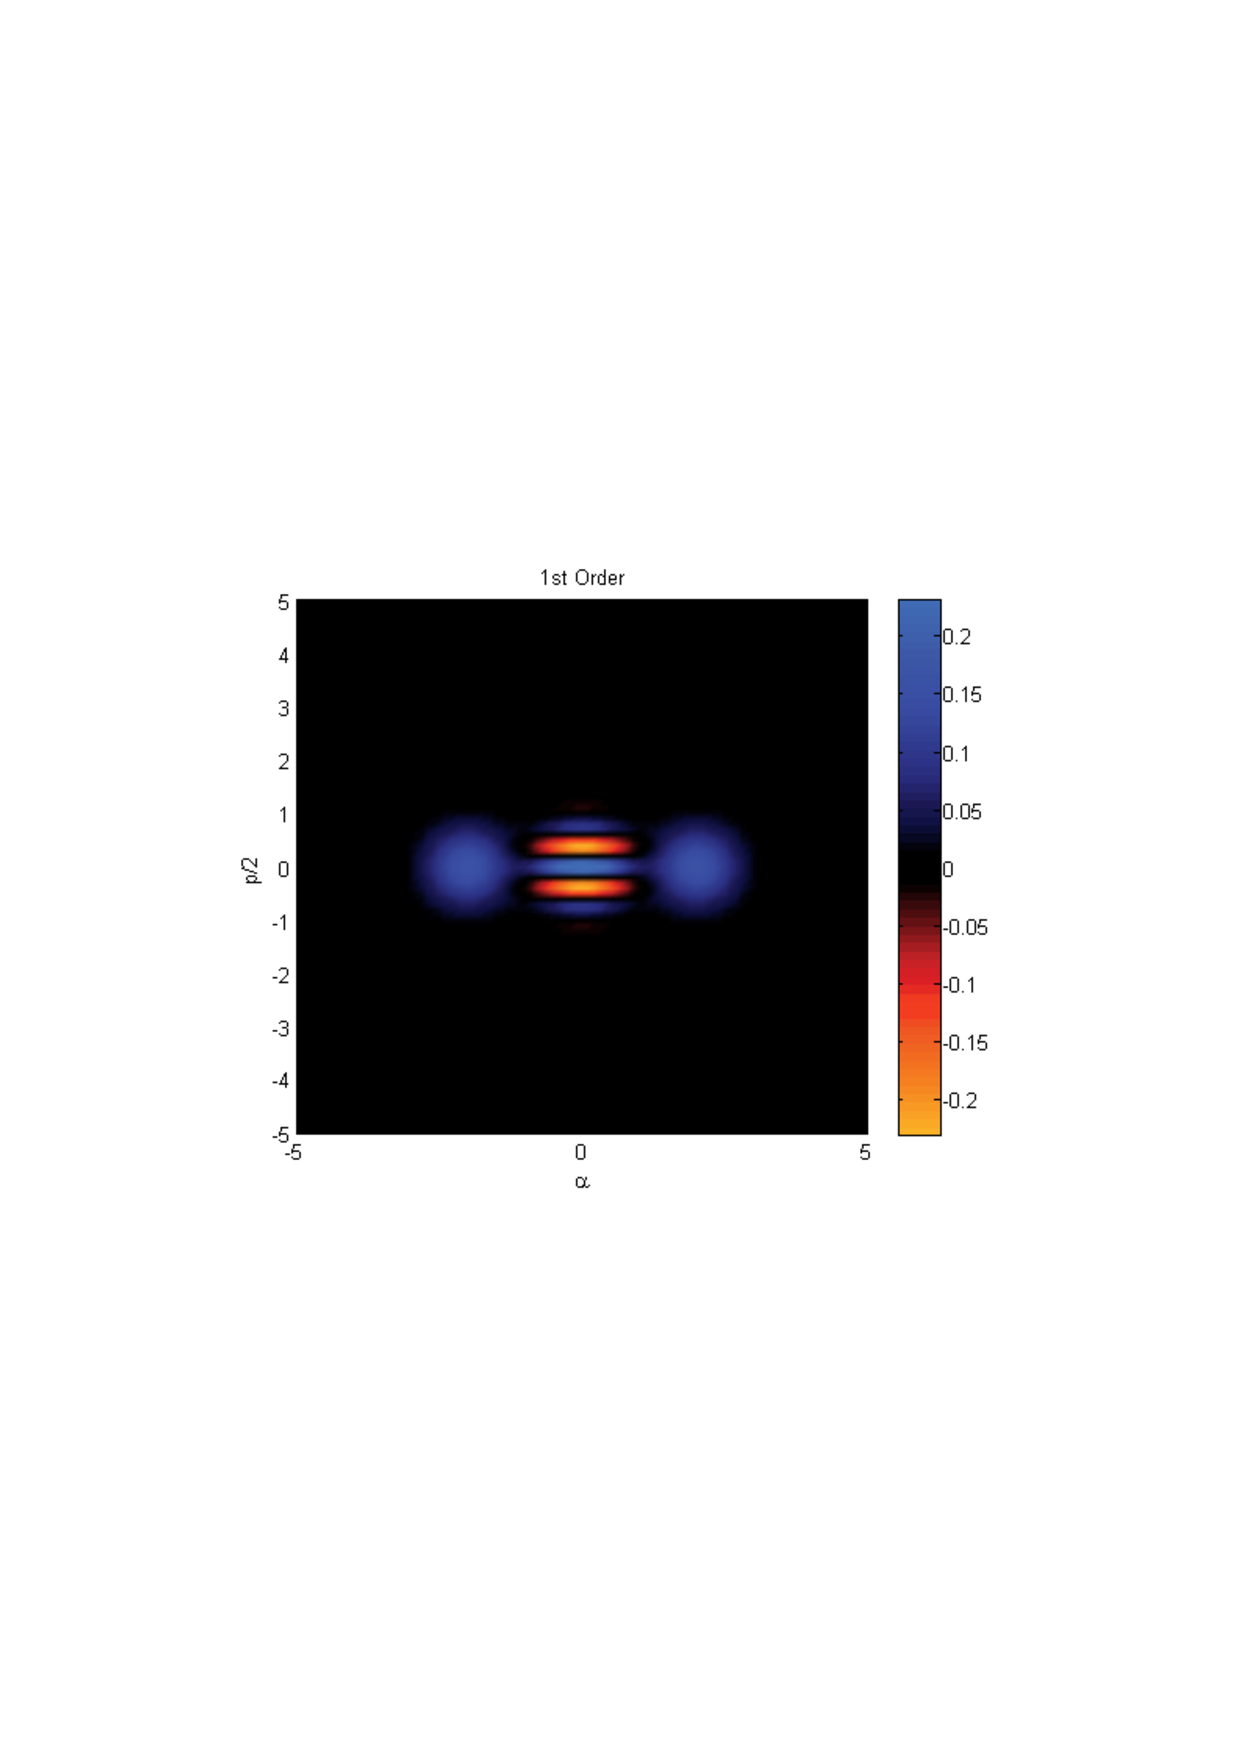
\includegraphics[scale=0.45]{1stOrder.pdf}\\
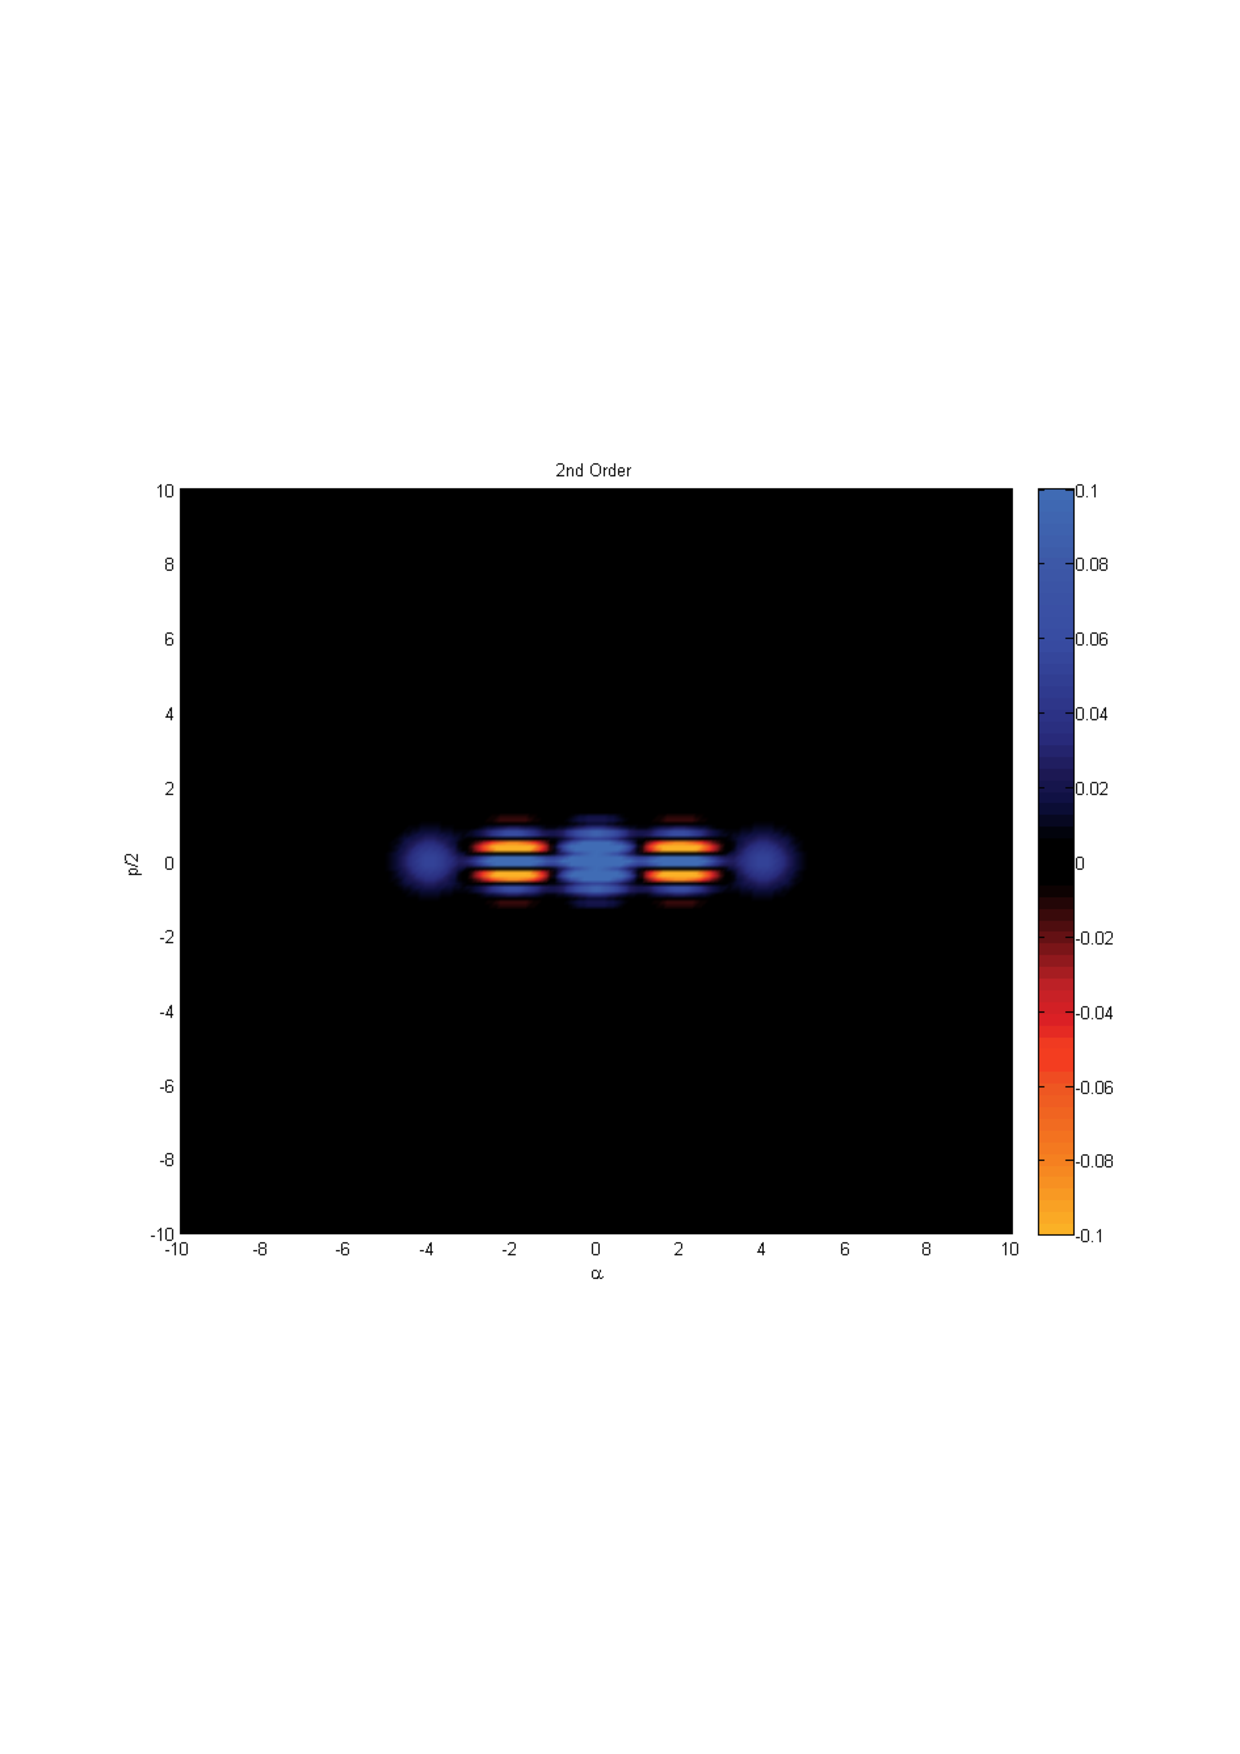
\includegraphics[scale=0.35]{2ndOrder.pdf}\\
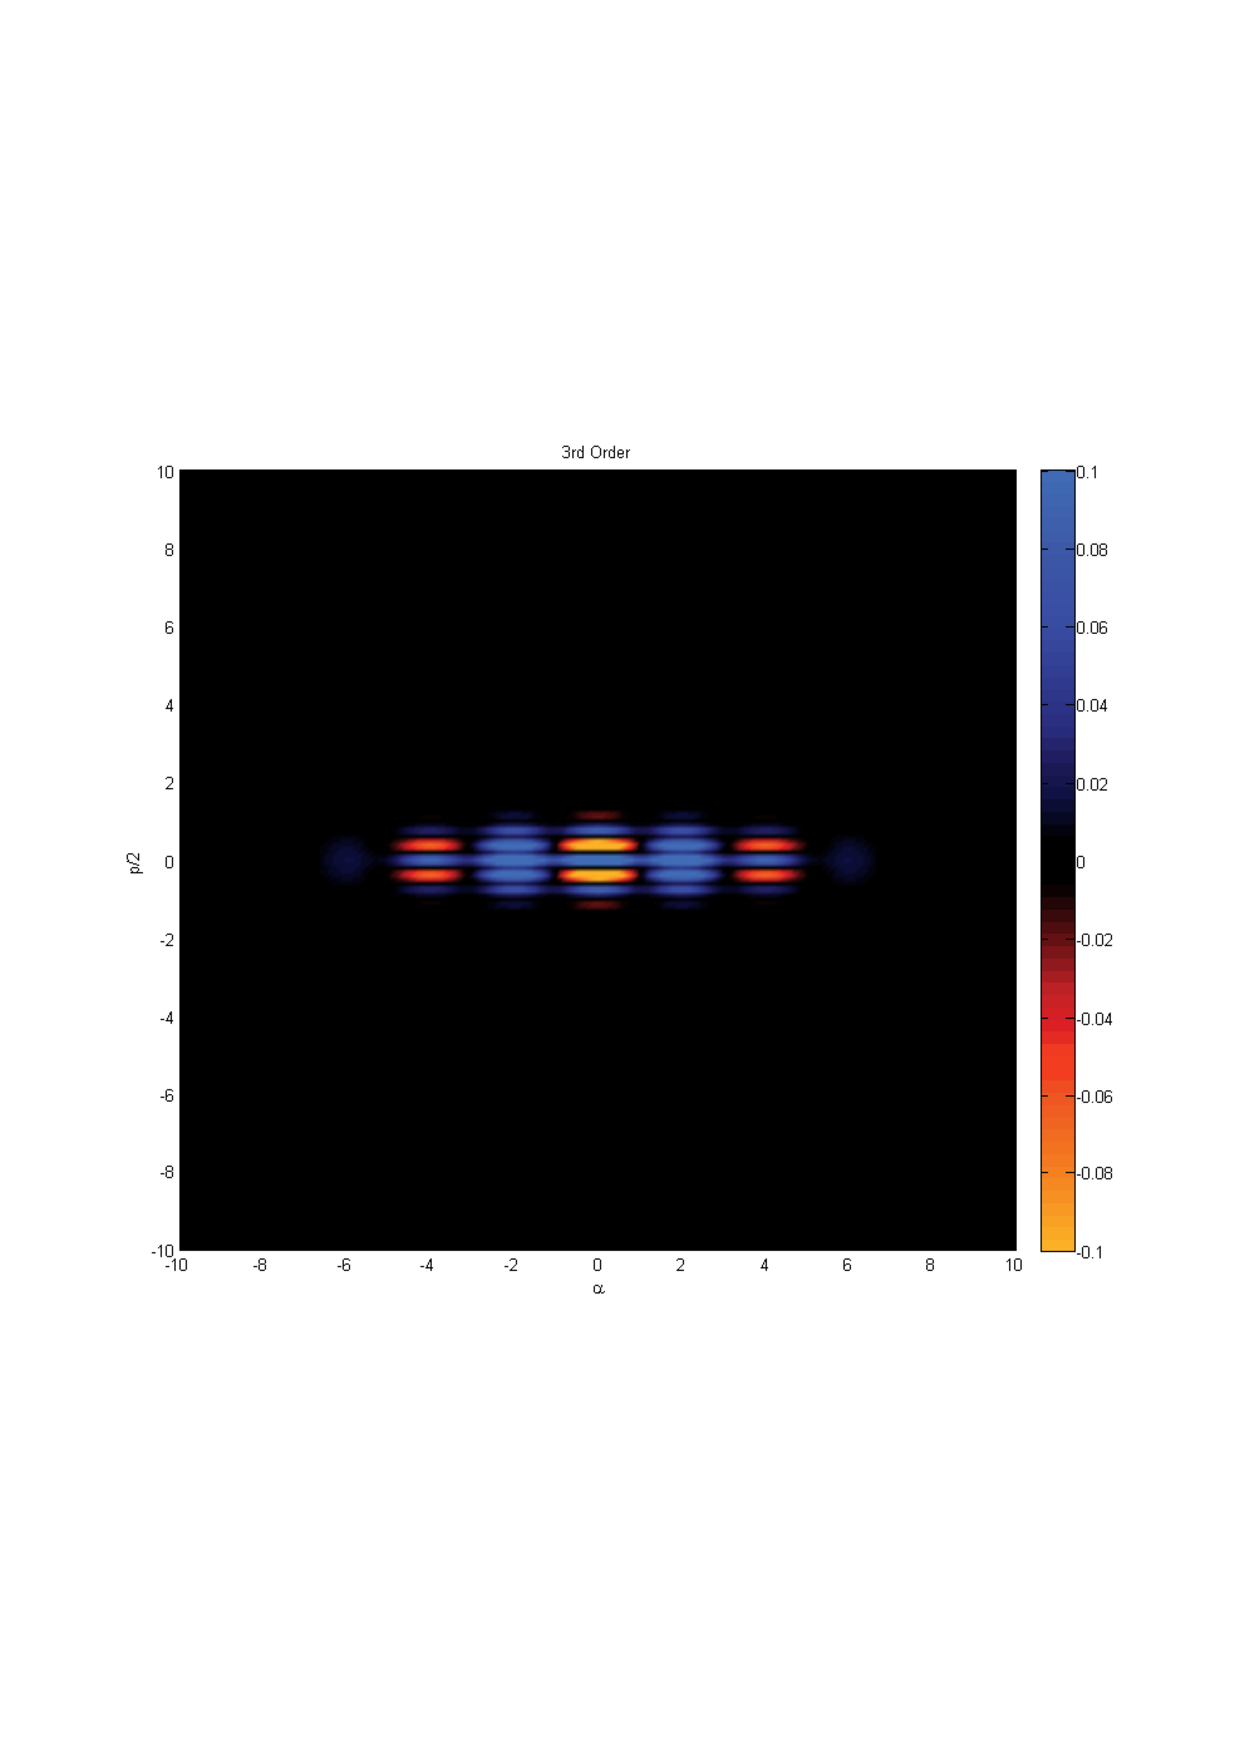
\includegraphics[scale=0.35]{3rdOrder.pdf}\\
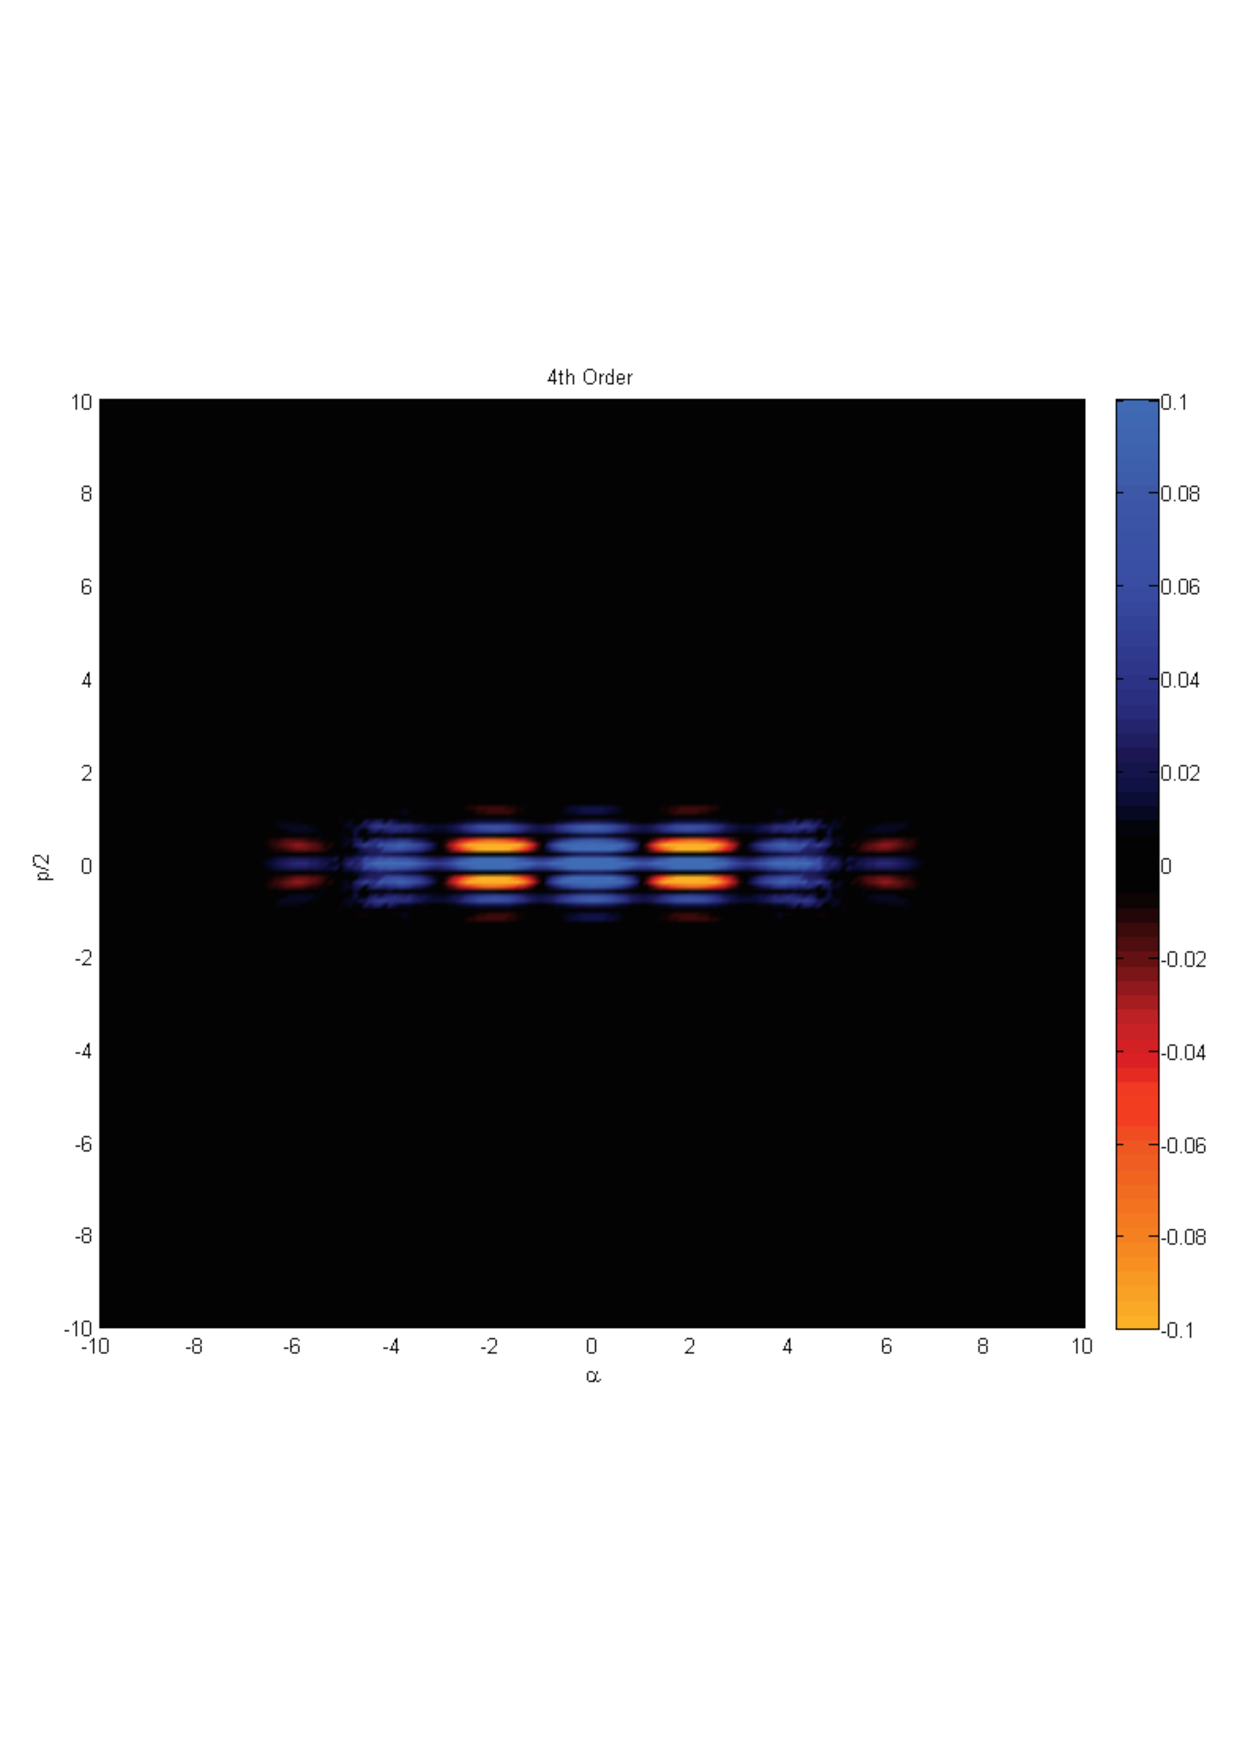
\includegraphics[scale=0.3]{4thOrder.pdf}
\caption{\label{fig:Cats}\keith{Wigner function of the (a) first $A^{\dag}_+(\alpha)$, (b) second $A^{\dag2}_+(\alpha)$, (c) third $A^{\dag3}_+(\alpha)$, and (d) fourth $A^{\dag4}_+(\alpha)$ order cat state for $\alpha=2$. The quantum signatures from the Wigner function oscillate in it's phase space  from even to odd ordered states.}}
\end{figure}
%***********************************

\subsection{Second Order Cats}
There are four combinations of how second order cats can be created
\begin{eqnarray} \label{eq:HOC1}
A^\dag_-(\alpha)A^\dag_-(\beta) &=& [D(\alpha)-D(-\alpha)][D(\beta)-D(-\beta)] \nonumber \\ 
&=& D(\alpha+\beta) + D(-\alpha-\beta) \nonumber \\ 
&&- D(\alpha-\beta) - D(-\alpha+\beta) \nonumber \\ 
&=& A^\dag_+(\alpha+\beta) - A^\dag_+(\alpha-\beta)
\end{eqnarray}

\begin{eqnarray} \label{eq:HOC2}
A^\dag_+(\alpha)A^\dag_+(\beta) &=& [D(\alpha)+D(-\alpha)][D(\beta)+D(-\beta)] \nonumber \\ 
&=& D(\alpha+\beta) + D(-\alpha-\beta) \nonumber \\ 
&&+ D(\alpha-\beta) + D(-\alpha+\beta) \nonumber \\ 
&=& A^\dag_+(\alpha+\beta) + A^\dag_+(\alpha-\beta)
\end{eqnarray}

\begin{eqnarray} \label{eq:HOC3}
A^\dag_+(\alpha)A^\dag_-(\beta) &=& [D(\alpha)+D(-\alpha)][D(\beta)-D(-\beta)] \nonumber \\ 
&=& D(\alpha+\beta) - D(-\alpha-\beta) \nonumber \\ 
&& -D(\alpha-\beta) + D(-\alpha+\beta) \nonumber \\ 
&=& A^\dag_-(\alpha+\beta) - A^\dag_-(\alpha-\beta)
\end{eqnarray}

\begin{eqnarray} \label{eq:HOC4}
A^\dag_-(\alpha)A^\dag_+(\beta) &=& [D(\alpha)-D(-\alpha)][D(\beta)+D(-\beta)] \nonumber \\ 
&=& D(\alpha+\beta) - D(-\alpha-\beta) \nonumber \\ 
&& +D(\alpha-\beta) - D(-\alpha+\beta) \nonumber \\ 
&=& A^\dag_-(\alpha+\beta) + A^\dag_-(\alpha-\beta)
\end{eqnarray}

When $\alpha=\beta$ these become,
\begin{eqnarray} \label{eq:sameSOC}
A^\dag_-(\alpha)A^\dag_-(\alpha) &=& A^\dag_+(2\alpha) - 2 \\
A^\dag_+(\alpha)A^\dag_+(\alpha) &=& A^\dag_+(2\alpha) + 2 \\
A^\dag_+(\alpha)A^\dag_-(\alpha) &=& A^\dag_-(2\alpha) \\
A^\dag_-(\alpha)A^\dag_+(\alpha) &=& A^\dag_-(2\alpha)
\end{eqnarray}
Thus, in general, a second order cat is a superposition of two first order cats of the sum and difference of the respective amplitudes. From these rules, one can recursively define the application of higher order cat creation operators in terms of superpositions of first order cat creation operators. Specifically, an $n$th power of the cat creation operator will be a superposition of $2^{n-1}$ first order cat creation operators. \keith{\textbf{Lets plot the +- \& -+ versions of the second order cats and it seems that you just get a first order cat because the vacuum term is not present. It's seems as though by acting the + and - or - and + maybe the order doesn't increase. But maybe something else interesting is happening. One interesting thing is that maybe it just grows the cat instead of increasing the order.}}


\keith{\subsection{Third Order Cats}
The third order cat,
\begin{eqnarray} \label{eq:HOC3}
A^\dag_+(\alpha)A^\dag_+(\beta)A^\dag_+(\gamma) &=& A^\dag_+(\alpha+\beta+\gamma) + A^\dag_+(-\alpha+\beta+\gamma) \nonumber \\ 
&+& A^\dag_+(\alpha-\beta+\gamma) + A^\dag_+(-\alpha-\beta+\gamma) \nonumber \\
\end{eqnarray}
is in general a superposition of four first order cat operators. Or this can be written in terms of two second order cats as,
\begin{eqnarray} \label{}
A^\dag_+(\alpha)A^\dag_+(\beta)A^\dag_+(\gamma) &=& A^\dag_+(\beta+\gamma+\alpha)A^\dag_+(\beta+\gamma-\alpha) \nonumber \\ 
&+& A^\dag_+(\gamma-\beta+\alpha)A^\dag_+(\gamma-\beta-\alpha),\nonumber \\
 \end{eqnarray}
 which can be written in terms of first order cats,
 \begin{eqnarray} \label{}
A^\dag_+(\alpha)A^\dag_+(\beta)A^\dag_+(\gamma) &=& A^\dag_+(2(\gamma+\beta))+A^\dag_+(2\alpha) \nonumber \\ 
&+& A^\dag_+(2(\gamma-\beta))+A^\dag_+(2\alpha) \nonumber \\
&=& A^\dag_+(2(\gamma+\beta)) + A^\dag_+(2(\gamma-\beta)) \nonumber \\
&+& 2A^\dag_+(2\alpha).
 \end{eqnarray}
This is in general a superposition of three first order cats.

When $\alpha=\beta=\gamma$ we get,
 \begin{eqnarray} \label{}
A^\dag_+(\alpha)A^\dag_+(\beta)A^\dag_+(\gamma) &=& A^\dag_+(4\alpha)+A^\dag_+(2\alpha)+2. \nonumber \\
\end{eqnarray}
}
\section{Beamsplitter rules}

Consider a two-port beamsplitter that implements the transformation,
\begin{eqnarray}
\left( \begin{array}{c}
a^\dag \\
b^\dag \\
\end{array} \right)
\to \left( \begin{array}{cc}
U_{1,1} & U_{1,2} \\
U_{2,1} & U_{2,2} \\
\end{array} \right)
\left( \begin{array}{c}
a^\dag \\
b^\dag \\
\end{array} \right)
\end{eqnarray}
In displacement operator language this is,
\begin{eqnarray}
D_1(\alpha) &\to& D_1(U_{1,1} \alpha) D_2(U_{1,2} \alpha) \nonumber \\
D_2(\alpha) &\to& D_1(U_{2,1} \alpha) D_2(U_{2,2} \alpha)
\end{eqnarray}
where subscript denotes mode number. That is, a beamsplitter maps a coherent state to a tensor product of coherent states.

Then it follows that
\begin{eqnarray}
A_\pm^\dag(\alpha) &=& [D_1(\alpha)\pm D_1(-\alpha)] \nonumber \\
&\to& D_1(U_{1,1}\alpha)D_2(U_{1,2}\alpha)\nonumber\\
&\pm& D_1(-U_{1,1}\alpha)D_2(-U_{1,2}\alpha) \nonumber \\
B_\pm^\dag(\alpha) &=& [D_2(\alpha)\pm D_2(-\alpha)] \nonumber \\
&\to& D_1(U_{2,1}\alpha)D_2(U_{2,2}\alpha)\nonumber\\
&\pm& D_1(-U_{2,1}\alpha)D_2(-U_{2,2}\alpha) \nonumber \\
\end{eqnarray}
where $A$ and $B$ are cat operators on the first and second output modes.

Thus,
\begin{eqnarray}
A_\pm^\dag(\alpha) &\to& A_+^\dag(U_{1,1} \alpha) B_\pm^\dag(\pm U_{1,2} \alpha) \nonumber\\
&\pm& A_-^\dag(U_{1,1} \alpha)B_\mp^\dag(\pm U_{1,2} \alpha) \nonumber \\
B_\pm^\dag(\alpha) &\to& A_+^\dag(U_{2,1} \alpha) B_\pm^\dag(\pm U_{2,2} \alpha) \nonumber\\
&\pm& A_-^\dag(U_{2,1} \alpha)B_\mp^\dag(\pm U_{2,2} \alpha)
\end{eqnarray}

\textbf{Double check this!}

Thus the beamsplitter maps a cat creation operator to a path entangled superposition of two first order cats of smaller amplitude.

\section{Breeding cats}

\textbf{This section needs the normalisations to be checked}

Let us prepare a 50/50 beamsplitter given by the Hadamard matrix,
\begin{eqnarray}
U = \frac{1}{\sqrt{2}} \left( \begin{array}{cc}
1 & 1 \\
1 & -1 \\
\end{array} \right)
\end{eqnarray}

with a first order cat state at each input, $A_+^\dag(\alpha)\otimes B_+^\dag(\alpha)\ket{0}_1 \ket{0}_2$. Then, using our beamsplitter relation we have,
\begin{eqnarray}
A_+^\dag(\alpha)\otimes B_+^\dag(\alpha)\ket{0}_1 \ket{0}_2 &\to&\frac{1}{2}\left[[A_+^\dag(\alpha/\sqrt{2}) B_+^\dag(\alpha/\sqrt{2}) \right.\nonumber \\
&+& A_-^\dag(\alpha/\sqrt{2}) B_-^\dag(\alpha/\sqrt{2})] \nonumber\\
&\times& [A_+^\dag(\alpha/\sqrt{2}) B_+^\dag(-\alpha/\sqrt{2}) \nonumber \\
&+& \left.A_-^\dag(\alpha/\sqrt{2})B_-^\dag(-\alpha/\sqrt{2})]\right]\ket{0}_1 \ket{0}_2 \nonumber \\
\end{eqnarray}
Upon expansion this yields,
\begin{eqnarray}
\frac{1}{2}\left[A_+^\dag(\alpha/\sqrt{2}) B_+^\dag(\alpha/\sqrt{2}) A_+^\dag(\alpha/\sqrt{2}) B_+^\dag(-\alpha/\sqrt{2}) \right. \nonumber \\
+ A_+^\dag(\alpha/\sqrt{2}) B_+^\dag(\alpha/\sqrt{2}) A_-^\dag(\alpha/\sqrt{2})B_-^\dag(-\alpha/\sqrt{2}) \nonumber \\
+ A_-^\dag(\alpha/\sqrt{2})B_-^\dag(\alpha/\sqrt{2}) A_+^\dag(\alpha/\sqrt{2}) B_+^\dag(-\alpha/\sqrt{2}) \nonumber \\
\left. + A_-^\dag(\alpha/\sqrt{2})B_-^\dag(\alpha/\sqrt{2})A_-^\dag(\alpha/\sqrt{2})B_-^\dag(-\alpha/\sqrt{2}) \right]\ket{0}_1 \ket{0}_2.\nonumber \\
\end{eqnarray}

Since the operators commute we can rewrite this as,
\begin{eqnarray}
\frac{1}{2}\left[A_+^\dag(\alpha/\sqrt{2}) A_+^\dag(\alpha/\sqrt{2}) B_+^\dag(\alpha/\sqrt{2})  B_+^\dag(-\alpha/\sqrt{2}) \right. \nonumber \\
+ A_+^\dag(\alpha/\sqrt{2}) A_-^\dag(\alpha/\sqrt{2}) B_+^\dag(\alpha/\sqrt{2}) B_-^\dag(-\alpha/\sqrt{2}) \nonumber \\
+ A_-^\dag(\alpha/\sqrt{2})A_+^\dag(\alpha/\sqrt{2})B_-^\dag(\alpha/\sqrt{2})  B_+^\dag(-\alpha/\sqrt{2}) \nonumber \\
\left.+ A_-^\dag(\alpha/\sqrt{2}) A_-^\dag(\alpha/\sqrt{2})B_-^\dag(\alpha/\sqrt{2})B_-^\dag(-\alpha/\sqrt{2})\right] \ket{0}_1 \ket{0}_2.\nonumber \\
\end{eqnarray}
According to Eq.'s \ref{eq:HOC1}, \ref{eq:HOC2}, \ref{eq:HOC3}, and \ref{eq:HOC4} the second order terms can be rewritten in terms of a superposition of first order terms. Applying this to the $B_{\pm}^{\dag}$ terms this becomes,
\begin{eqnarray}
\frac{1}{2}\left[A_+^\dag(\alpha/\sqrt{2}) A_+^\dag(\alpha/\sqrt{2}) \left(B_+^\dag(0)+  B_+^\dag(\sqrt{2}\alpha)\right) \right.\nonumber \\
+ A_+^\dag(\alpha/\sqrt{2}) A_-^\dag(\alpha/\sqrt{2}) \left(B_-^\dag(0)-  B_-^\dag(\sqrt{2}\alpha)\right) \nonumber \\
+ A_-^\dag(\alpha/\sqrt{2})A_+^\dag(\alpha/\sqrt{2})\left(B_-^\dag(0)+  B_-^\dag(\sqrt{2}\alpha)\right) \nonumber \\
\left.+ A_-^\dag(\alpha/\sqrt{2}) A_-^\dag(\alpha/\sqrt{2})\left(B_+^\dag(0)-  B_+^\dag(\sqrt{2}\alpha)\right)\right]\ket{0}_1 \ket{0}_2.\nonumber \\
\end{eqnarray}

Let us post-select upon detecting the vacuum state at the second output mode. Then the odd cat terms in the second mode, $B_-^\dag$, vanish, as they only contain odd photon number terms and never $\ket{0}$. The remaining terms are,
%By using the projector $\ket{0}\bra{0}$
\begin{eqnarray}
\frac{1}{\sqrt{2}}\bra{0}_2\left[A_+^\dag(\alpha/\sqrt{2}) A_+^\dag(\alpha/\sqrt{2}) \left(B_+^\dag(0)+  B_+^\dag(\sqrt{2}\alpha)\right) \right.\nonumber \\
\left.+ A_-^\dag(\alpha/\sqrt{2}) A_-^\dag(\alpha/\sqrt{2})\left(B_+^\dag(0)-  B_+^\dag(\sqrt{2}\alpha)\right)\right]\ket{0}_1 \ket{0}_2 .\nonumber \\
\end{eqnarray}
Projecting $\bra{0}_2$ will pull out the $\ket{0}$ photon amplitudes of the remainding $B_+^{\dag}$ terms, which leaves us with
\begin{eqnarray}
\frac{1}{\sqrt{2}}\left[A_+^\dag(\alpha/\sqrt{2}) A_+^\dag(\alpha/\sqrt{2}) \left(2+ c_1\right) \right.\nonumber \\
\left.+ A_-^\dag(\alpha/\sqrt{2}) A_-^\dag(\alpha/\sqrt{2})\left(2-  c_1)\right)\right]\ket{0}_1 \ket{0}_2,\nonumber \\
\end{eqnarray}
where \keith{$c_1\propto2e^{-|\alpha|^2}$} is the corresponding amplitude of the $\ket{0}$ term in the $B_+^\dag(\sqrt{2}\alpha)$ cat state. 

After expanding this out in terms of first order cats and simplifying we obtain,
\begin{eqnarray}
2\sqrt{2}\left[A_+^\dag(\sqrt{2}\alpha)+c_1\right]\ket{0}_1 \nonumber \\
=2\sqrt{2}\left[A_+^\dag(\sqrt{2}\alpha)+2e^{-|\alpha|^2}\right]\ket{0}_1
\end{eqnarray}
which looks like a second order cat as in Eq. \ref{eq:sameSOC} but with a smaller vacuum component.

Thus, a beamsplitter fed with two first order cat states, conditioned upon the vacuum state at one output, yields a second order cat state, providing a simple experimental prescription for preparing higher-order cat states.

\textbf{Generalise this result to breeding arbitrary higher order cat states. i.e. let's show that we can make an $n+1$ order cat state from an $n$ order cat state and a first order cat states. Then it will follow recursively that we can generate cats of arbitrary order.}

%\begin{acknowledgments}
%This research was conducted by the Australian Research Council Centre of Excellence for Engineered Quantum Systems (Project number CE110001013). 
%\end{acknowledgments}

\bibliography{paper}

\end{document}
